As illustrated in the system overview (Figure~\ref{fig:system_overview}), the Apache Kafka cluster is crucial to the system architecture, serving as a real-time messaging backbone between CPU-based edge devices and the centralized server. Kafka ensures efficient, reliable, and scalable data streaming, effectively mitigating several potential critical issues inherent to direct edge-server communication:

\begin{itemize}
\item \textbf{Bottleneck}: A bottleneck refers to a point in a system that restricts overall performance due to limited throughput capabilities. In practical scenarios, each edge device streams data at an average rate of 12-20 FPS. Thus, with just 10 devices, the centralized server receives approximately 120-200 messages per second. This volume of messages can quickly exceed the server's processing capacity, even when supported by powerful hardware.

Additionally, network bandwidth becomes a significant constraint. For instance, at 12~FPS with each message roughly 1~MB in size (including FullHD video frames, bounding box coordinates, and metadata such as frame ID and timestamps), the server processes about 12~MB/s per device. Consequently, a system of 10~devices generates approximately 120~MB/s (0.96 Gbps), necessitating extremely high and stable bandwidth to prevent congestion.

Kafka alleviates these bottlenecks by buffering and efficiently distributing message loads, allowing smooth and reliable server processing.

\item \textbf{Loss of Data}: Without Kafka, edge devices would directly transmit data to the centralized server, posing risks of significant data loss due to network disruptions (such as weather interference or intermittent connectivity). Kafka's design inherently provides message durability through its distributed log structure, ensuring that messages are stored persistently until successfully processed, thus greatly reducing potential data loss.

\item \textbf{Synchronization}: Direct edge-server communication would necessitate complex synchronization mechanisms to maintain the correct order of frames, a critical requirement for accurate tracking in Re-ID applications. Kafka inherently ensures ordered message processing by managing partitioned logs effectively. Thus, it simplifies synchronization significantly, guaranteeing the sequential integrity of frames from each camera source.

\end{itemize}

Due to these critical considerations, Apache Kafka plays an indispensable role, providing robust, efficient, and reliable data management essential for the seamless operation of the Re-ID pipeline.

\subsection{Cluster configuration}

A Kafka cluster is a collection of multiple Kafka brokers that work together, managed by a single Zookeeper node or a cluster of Zookeeper nodes. Based on the properties of the current Re-ID system, a cluster includes three brokers and one Zookeeper node is selected to ensure high availability and fault tolerance, as illustrated in Figure~\ref{fig:kafka_cluster}.

\begin{figure}[htbp]
    \centering
    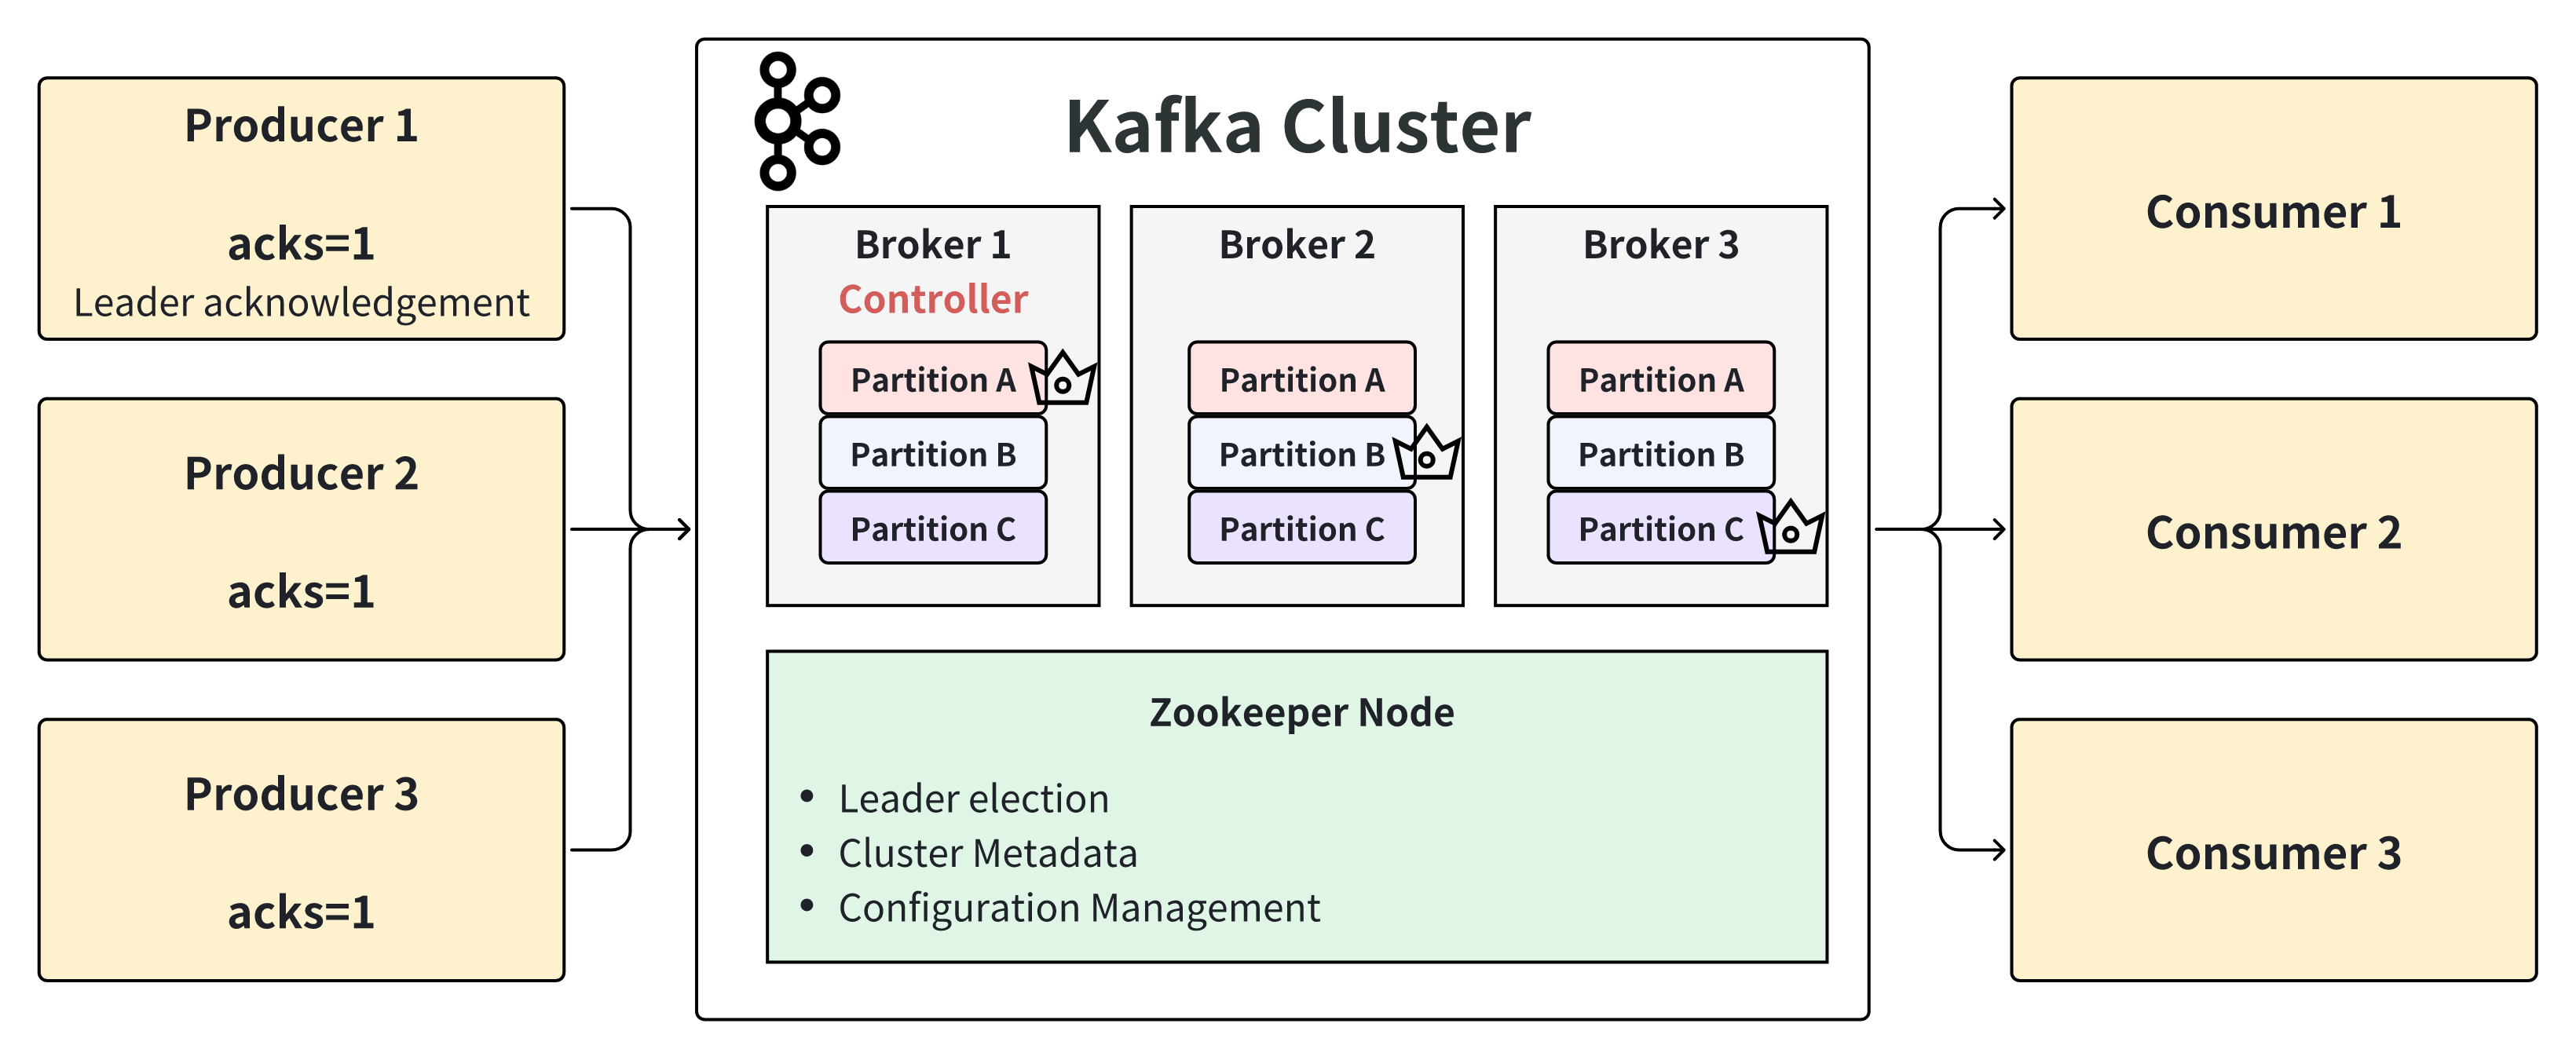
\includegraphics[width=1\textwidth]{Figure/kafka_overview.png}
    \caption{Kafka clusters with three brokers and one Zookeeper node.}
    \label{fig:kafka_cluster}
\end{figure}

\paragraph{Zookeeper node}

The Zookeeper service manages cluster metadata, including broker registration, topic configuration, partition leadership information, and consumer group coordination. It ensures consistent configuration management across the entire Kafka ecosystem.

\paragraph{Kafka brokers}

The three Kafka brokers (Broker 1, Broker 2, and Broker 3) form the core of the Kafka cluster, as depicted in Figure~\ref{fig:kafka_cluster}. These brokers are responsible for storing data, managing message partitions, and enabling communication between producers and consumers. Each broker hosts different partitions of the data topics:

\begin{itemize}
    \item \textit{Controller}: One broker acts as the cluster controller. The controller handles administrative tasks such as assigning partitions to brokers, managing leadership elections for partitions, and monitoring the overall cluster state.
    
    \item \textit{Topics}: Topics represent logical streams of records categorized by specific names, serving as the fundamental organizational unit for data flow within Kafka. While topics are conceptual abstractions rather than physical entities, they provide essential structure for message categorization and routing. In the context of this Re-ID system, topics such as \texttt{reid\_input} are used to channel video frame data and metadata from edge devices to the centralized server. Each topic can accommodate multiple producers (edge devices) simultaneously writing data and multiple consumers (server-side processing modules) reading data, enabling flexible many-to-many communication patterns essential for scalable distributed processing.
    
    \item \textit{Partitions}: Each topic is divided into partitions (based on initial setup) to facilitate scalability and parallelism. In Figure~\ref{fig:kafka_cluster}, these partitions are distributed across the three brokers, with each partition having a designated leader (marked by a crown icon). The leader partition is responsible for managing read and write requests from producers and consumers. Follower partitions serve as replicas to ensure data redundancy and fault tolerance.
\end{itemize}

\paragraph{Producers and Consumers}

The system includes multiple producers representing the edge devices that send messages to the Kafka cluster with an acknowledgment setting of \texttt{acks=1}, meaning producers wait for confirmation only from the leader broker before proceeding. On the consumer side, multiple consumers subscribe to Kafka topics to read and process data. Messages from partitions are delivered to consumers based on their subscription configuration and current offset position.

The coordination of these distributed producers and consumers, along with the management of broker leadership and partition assignments, requires a centralized coordination service. This critical orchestration role is fulfilled by Apache ZooKeeper, which serves as the backbone for maintaining cluster metadata and ensuring consistent distributed state management across all Kafka components.

To comprehensively understand the operational mechanics of the Kafka cluster within this Re-ID system, it is essential to examine the following fundamental concepts and their specific implementations:

\subsection{Zookeeper node}

In this Re-ID system, we use a single Zookeeper node instead of the common 3-node ensemble. This choice is based on the system's needs and practical reasons:

\begin{itemize}
    \item \textbf{Resource Efficiency}: For the current scale (3 Kafka brokers with moderate message flow), one Zookeeper node is enough to manage coordination without wasting extra computing power or network resources that could be used by the Re-ID system itself.
    
    \item \textbf{Simpler Management}: Having a single node reduces complexity, which is helpful for small to medium enterprises (SMEs) that may not have dedicated DevOps staff. It also makes monitoring, backups, and troubleshooting easier.
    
    \item \textbf{Development and Testing}: This setup works well for development, testing, and early production stages where quick deployment and cost saving are more important than full availability.
\end{itemize}

For larger or more critical deployments, it is easy to switch to a 3-node Zookeeper ensemble to improve reliability.

\paragraph{Partition Assignment and Producer Acknowledgement}

As configured, the producer's acknowledgment setting is \texttt{acks = 1}, which means the producer waits for a confirmation only from the leader partition before considering the message successfully sent. This setting provides a balance between latency and data safety, allowing faster message delivery while ensuring that the leader has safely written the message.

For partition assignment, Kafka uses a round-robin strategy when no specific key is provided. For the \texttt{reid\_input} topic with 6 partitions, the partition ID for the \(i\)-th message is determined by:

\begin{equation}
    \text{Partition ID} = i \bmod 6, \quad i = 0, 1, 2, \ldots
\end{equation}

This ensures messages are evenly distributed across all partitions in a cyclic manner:

\[
0, 1, 2, 3, 4, 5, 0, 1, 2, \ldots
\]

Thus, with \texttt{acks = 1}, the producer receives acknowledgment as soon as the leader partition confirms the message write, optimizing throughput while maintaining reasonable reliability.

\paragraph{Leader Partition Election}

Kafka's leader election mechanism ensures high availability and fault tolerance through the following process:

\begin{enumerate}
    \item \textbf{Initial Leader Assignment}: When a topic is created, Kafka automatically assigns one replica as the leader for each partition. The controller broker (Broker 1 in this configuration) manages this initial assignment based on the replica placement strategy.
    
    \item \textbf{In-Sync Replica (ISR) Maintenance}: The leader maintains a list of In-Sync Replicas that are fully caught up with the leader's log. Only ISR members are eligible for leadership.
    
    \item \textbf{Leader Failure Detection}: Zookeeper monitors broker health through heartbeat mechanisms. When a leader becomes unavailable, the controller broker detects this failure.
    
    \item \textbf{New Leader Selection}: The controller selects a new leader from the ISR list, typically choosing the first available replica in the preferred replica list to maintain optimal load distribution.
    
    \item \textbf{Metadata Update}: Once a new leader is elected, the controller updates the cluster metadata and notifies all brokers and clients about the leadership change.
\end{enumerate}

This election process typically completes within seconds, ensuring minimal disruption to the Re-ID data processing pipeline.

\subsection{Kafka brokers}

The Kafka message broker cluster serves as the communication backbone between edge devices and the centralized server in the distributed Re-ID system. This section details the broker configuration, message serialization strategies, and the rationale behind our architectural decisions.

\subsubsection{Broker configuration and topology}

The proposed Kafka cluster employs a three-broker architecture deployed within a containerized environment using Docker, strategically designed to achieve optimal fault tolerance while maintaining resource efficiency for SME deployments. This distributed topology addresses the critical requirements of real-time person Re-ID systems through carefully orchestrated broker configurations and message flow patterns.

The cluster architecture incorporates the following key specifications:

\begin{itemize}
   \item \textbf{Broker Count}: Three strategically distributed brokers (Broker 1, Broker 2, Broker 3) provide high availability through redundancy while maintaining cost-effectiveness. This configuration enables the system to continue operating even with single-broker failures, ensuring uninterrupted Re-ID processing. The broker count can be dynamically scaled based on edge device proliferation and processing demands.
   \item \textbf{Replication Factor}: Critical topics maintain a replication factor of 3, ensuring complete data redundancy across all brokers. This configuration guarantees zero data loss during broker failures and enables seamless failover mechanisms for continuous operation.
   \item \textbf{Topic Partitioning}: The primary \texttt{reid\_input} topic is strategically partitioned into 6 segments, enabling parallel processing capabilities and intelligent load distribution across multiple consumer instances. This partitioning strategy maximizes throughput while maintaining message ordering within individual partitions.
   \item \textbf{Containerization}: Each broker operates within isolated Docker containers, providing deployment flexibility, horizontal scaling capabilities, and simplified maintenance operations. This containerized approach facilitates rapid deployment across diverse infrastructure environments.
\end{itemize}

The broker configuration is specifically optimized for video data transmission characteristics inherent to Re-ID applications. Each broker maintains sufficient memory allocation to handle the buffering of compressed video frames, accommodating message sizes ranging from 200-400 KB depending on scene complexity, motion dynamics, and compression algorithms. The configuration prioritizes both message throughput and reliability, incorporating adaptive batching mechanisms and optimized serialization protocols to minimize latency while ensuring data integrity throughout the Re-ID processing pipeline.

\subsubsection{Message serialization}
\label{sec:message_serialization}

In distributed Re-ID systems where edge devices communicate with central servers through Apache Kafka, a critical challenge emerges: efficiently encoding messages that contain both structured metadata and binary image data. The fundamental issue stems from the need to serialize heterogeneous data types—including device identifiers, detection results, timestamps, and raw image frames—into a single message format suitable for network transmission.

The primary constraint lies in the incompatibility between text-based serialization formats and binary data representation. Traditional approaches require careful consideration of encoding overhead, transmission efficiency, and system scalability.

\textbf{Baseline Approach: Base64 Encoding with JSON}

The conventional solution involves converting binary image data to Base64 encoding before embedding it within a JSON structure. This approach follows a four-step process:

\begin{enumerate}
    \item \textbf{Binary-to-Text Conversion}: Raw image data is encoded using Base64 algorithm to produce ASCII string representation
    \item \textbf{JSON Structure Formation}: The Base64 string is embedded as a field value within the JSON message structure containing metadata
    \item \textbf{Serialization}: The complete JSON object is serialized to bytes for network transmission
    \item \textbf{Kafka Transmission}: The encoded message is sent through Kafka topics
\end{enumerate}

The JSON message structure with base64 encoded image data follows this format:

\begin{figure}[htbp]
    \centering
    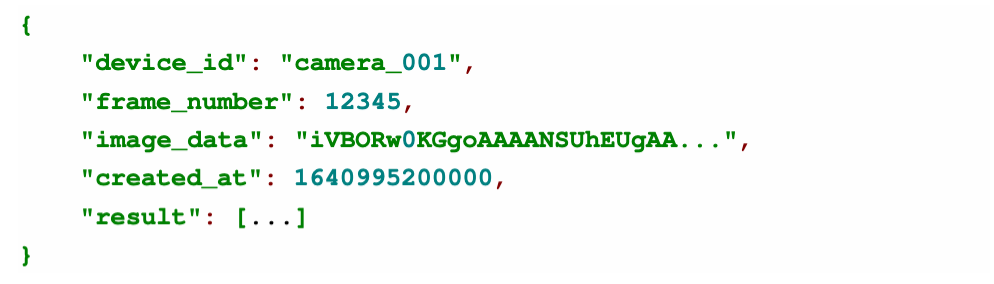
\includegraphics[width=1\textwidth]{Figure/json_base64.png}
    \caption{JSON message structure with Base64 encoded image data.}
    \label{fig:json_base64}
\end{figure}

This encoding is necessary because JSON, being a text-based format, cannot natively represent binary data. JSON supports only primitive types (string, number, boolean) and structural types (object, array), making text encoding the only viable option for binary data inclusion.

However, this approach introduces significant overhead. For a typical Full HD image frame with an original size of 2MB, the Base64 encoding process increases the message size to approximately 3MB—a 50\% increase. This expansion occurs due to Base64's inherent 33\% size inflation factor, compounded by JSON structural overhead.


To address the limitations of text-based encoding, we propose using Apache Avro as the primary serialization framework. Avro can be conceptualized as a binary equivalent of JSON that natively supports raw binary data without requiring text encoding, and also provide schema validation capabilities.

\textbf{Key Advantages}:
\begin{itemize}
    \item \textbf{Native Binary Support}: Direct handling of binary data without Base64 conversion
    \item \textbf{Apache Ecosystem Compatibility}: Seamless integration with Kafka, Schema Registry, and related tools
    \item \textbf{Schema Evolution}: Built-in support for backward and forward compatibility
    \item \textbf{Cross-Language Support}: Language-agnostic serialization format
\end{itemize}

The Avro schema definition for our edge device messages is structured as follows:

\newpage

\begin{figure}[htbp]
    \centering
    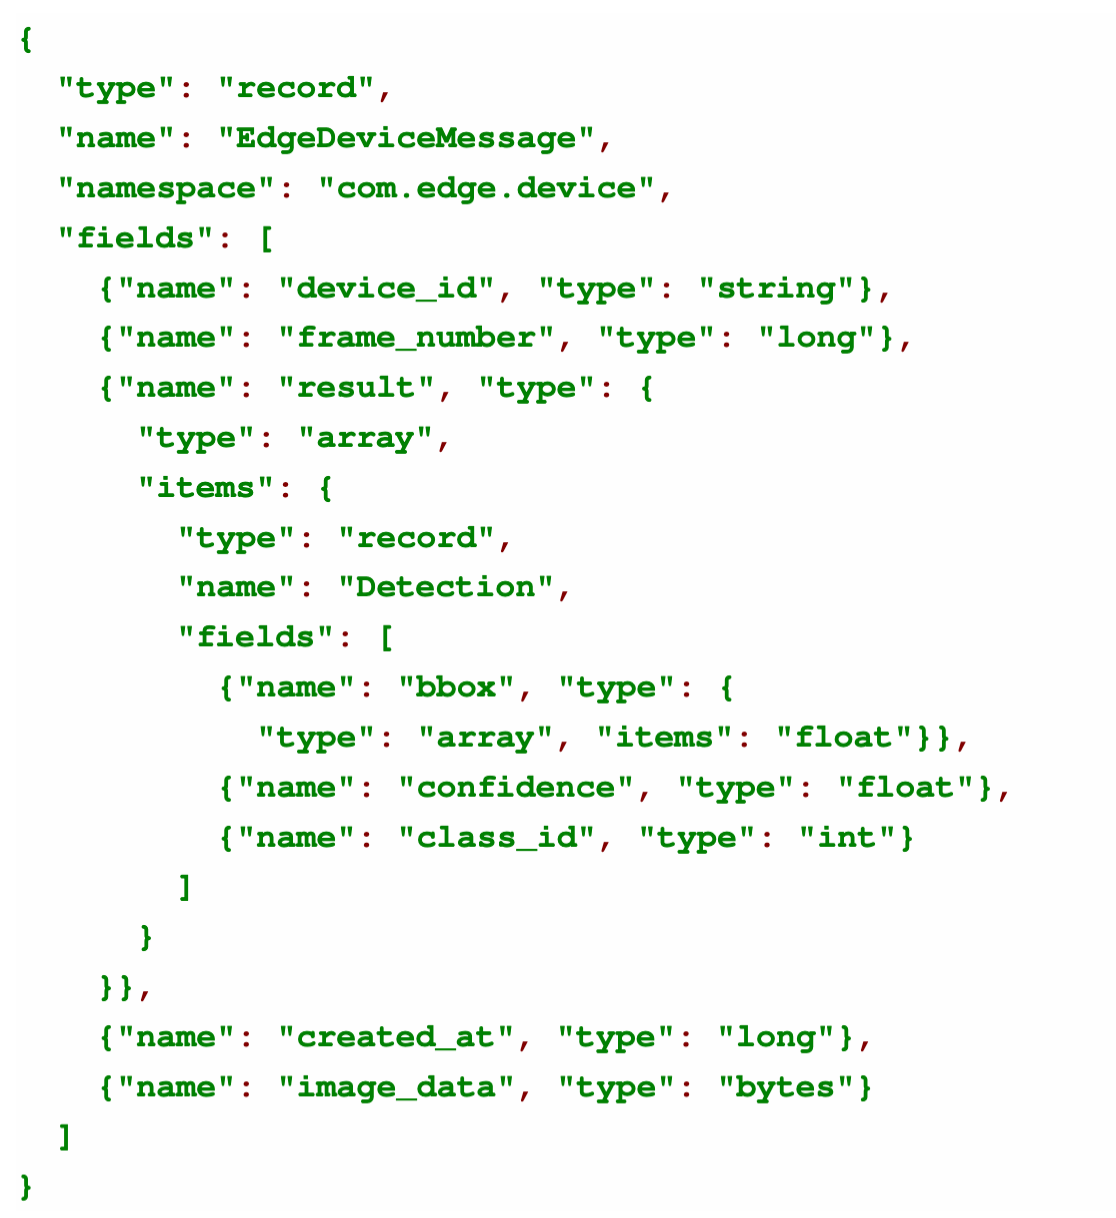
\includegraphics[width=0.8\textwidth]{Figure/avro_def.png}
    \caption{Avro schema definition for edge device messages.}
    \label{fig:avro_schema}
\end{figure}


\subsubsection{Topic settings}

In this project, two topics are used to facilitate the communication between edge devices and the centralized server:

\begin{itemize}
    \item \texttt{reid\_input}: The topic for edge devices to send messages to the Kafka cluster. On server side, each consumer will be assigned to a different consumer group to process different partitions of the topic, hence ensure that each consumer group will only fetch data from one  partition (one camera). 
    
    Below code shows the topic settings for \texttt{reid\_input}:
    
    \begin{lstlisting}[language=yaml]
    number_of_partitions: 6
    replication_factor: 3
    min_insync_replicas: 2
    cleanup_policy: delete
    retention_time: 1 day
    max_size_on_disk: 20 GB
    max_message_size: 20 MB
    \end{lstlisting}

    The \texttt{replication\_factor = 3} and \texttt{min\_insync\_replicas = 2} configuration ensures robust fault tolerance and high availability for the Re-ID system. With a replication factor of 3, each partition maintains three copies (one leader and two followers) distributed across the three Kafka brokers. This configuration can tolerate the failure of one broker without data loss or service interruption.
    
    For example, consider Partition 0 of the \texttt{reid\_input} topic:
    \begin{itemize}
        \item \textbf{Leader}: Broker 1 (handles all read/write operations)
        \item \textbf{Follower 1}: Broker 2 (maintains synchronized replica)
        \item \textbf{Follower 2}: Broker 3 (maintains synchronized replica)
    \end{itemize}
    
    The \texttt{min\_insync\_replicas = 2} setting requires that at least 2 replicas (leader + 1 follower) must acknowledge each write operation before considering it successful. This ensures that even if one broker fails, the data remains available and consistent. For instance:
    
    \textbf{Normal Operation}: All 3 replicas are in-sync, writes are acknowledged by leader + 1 follower.
    
    \textbf{Single Broker Failure}: If Broker 3 fails, Partition 0 still operates normally with Broker 1 (leader) and Broker 2 (follower) maintaining the minimum 2 in-sync replicas.
    
    \textbf{Critical Failure Scenario}: If 2 brokers fail simultaneously, the partition becomes read-only to prevent data inconsistency, ensuring data integrity over availability.
    
    \item \texttt{reid\_output}: The topic for storing processed frames with comprehensive metadata including person identifications, bounding boxes, and descriptive text annotations. This enables the client-side web application to interactively buffer and visualize real-time Re-ID results for users, providing a seamless interface for monitoring person tracking across the camera network.
    
    \begin{lstlisting}[language=yaml]
    number_of_partitions: 3
    replication_factor: 3
    min_insync_replicas: 2
    cleanup_policy: delete
    retention_time: 6 hours
    max_size_on_disk: 5 GB
    max_message_size: 10 MB
    \end{lstlisting}
    
    The \texttt{reid\_output} topic is configured with fewer partitions (three and six respectively) since output messages are typically aggregated results with lower frequency compared to continuous video frame input. The reduced retention time (six hours vs one day) reflects the time-sensitive nature of Re-ID results, where older identification data becomes less relevant for real-time tracking applications. The smaller maximum message size (10 MB vs 20 MB) accommodates processed metadata and identity vectors rather than raw video frames.
\end{itemize}

\subsection{Producers}

The Kafka producer configuration is essential for achieving efficient and reliable message delivery from edge devices to the Kafka cluster. Configuration parameters are optimized for the Re-ID system's real-time streaming requirements, balancing performance, data integrity, and system reliability.

\begin{figure}[htbp]
    \centering
    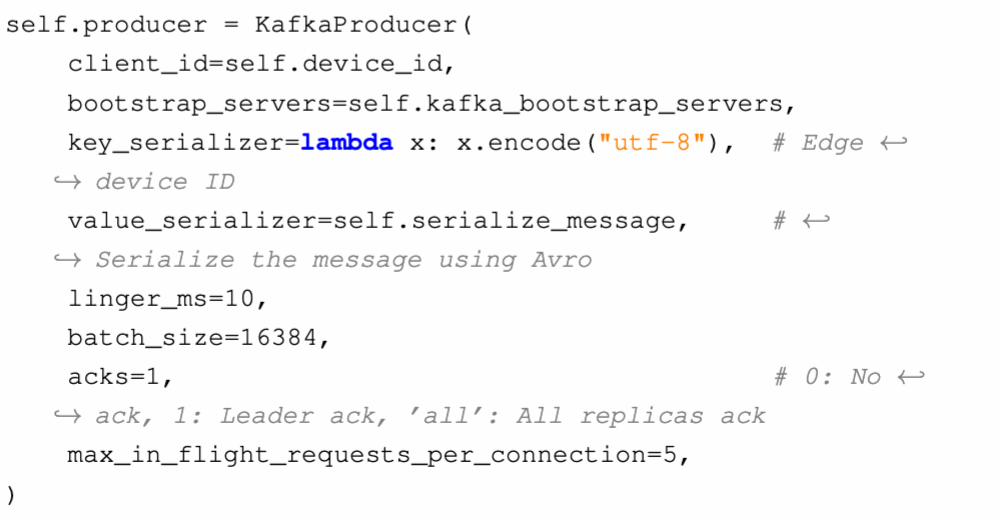
\includegraphics[width=0.9\textwidth]{Figure/producer_conf.png}
    \caption{Kafka producer configuration for edge devices.}
    \label{fig:producer_config}
\end{figure}

The producer configuration parameters are strategically chosen to balance throughput, latency, and reliability for the Re-ID streaming pipeline:

\begin{itemize}
    \item \textbf{client\_id}: Uniquely identifies each edge device producer within the Kafka cluster using the device ID. This facilitates monitoring, debugging, and tracking message flow from specific devices through the Kafka UI and broker logs.
    
    \item \textbf{bootstrap\_servers}: Specifies the initial list of Kafka broker addresses for establishing cluster connectivity. The producer uses this list to discover the full cluster topology and partition leadership information.
    
    \item \textbf{key\_serializer}: Serializes the message key (device ID) as UTF-8 encoded strings. The key serves dual purposes: ensuring message ordering per device and enabling consistent partition assignment for load balancing across the cluster.
    
    \item \textbf{value\_serializer}: Employs a custom Avro-based serialization function that efficiently encodes both structured metadata and binary image data without the overhead of text-based encoding schemes like Base64.
    
    \item \textbf{linger\_ms = 10}: Introduces a minimal 10-millisecond delay before sending batches, allowing the producer to collect multiple messages for batch transmission. This significantly improves network utilization and throughput while maintaining sub-frame latency for real-time processing.
    
    \item \textbf{batch\_size = 16384 bytes (16KB)}: Sets the maximum batch size for grouping messages before transmission. This value is optimized for the typical message size in our Re-ID system, where each message contains compressed image data and detection results.
    
    \item \textbf{acks = 1}: Configures acknowledgment requirements to wait only for the partition leader's confirmation before considering a message successfully sent. This provides an optimal balance between delivery guarantees and latency, suitable for near real-time applications where occasional message loss is acceptable.
    
    \item \textbf{max\_in\_flight\_requests\_per\_connection = 5}: Allows up to 5 unacknowledged requests per broker connection, enabling pipeline parallelism while preserving message ordering within each partition. This setting optimizes throughput without compromising the sequential nature of video frame processing.
\end{itemize}

This configuration ensures optimal performance for the Re-ID system's streaming requirements, achieving high throughput for continuous video frame processing while maintaining low latency for real-time person tracking and identification tasks.

\subsection{Consumers}

Similar to the producer configuration, the Kafka consumer setup requires common connectivity parameters. However, consumers also need additional specialized settings tailored explicitly for efficiently managing high-volume video streams and computationally demanding Re-ID processing tasks on the centralized server.

\begin{figure}[htbp]
    \centering
    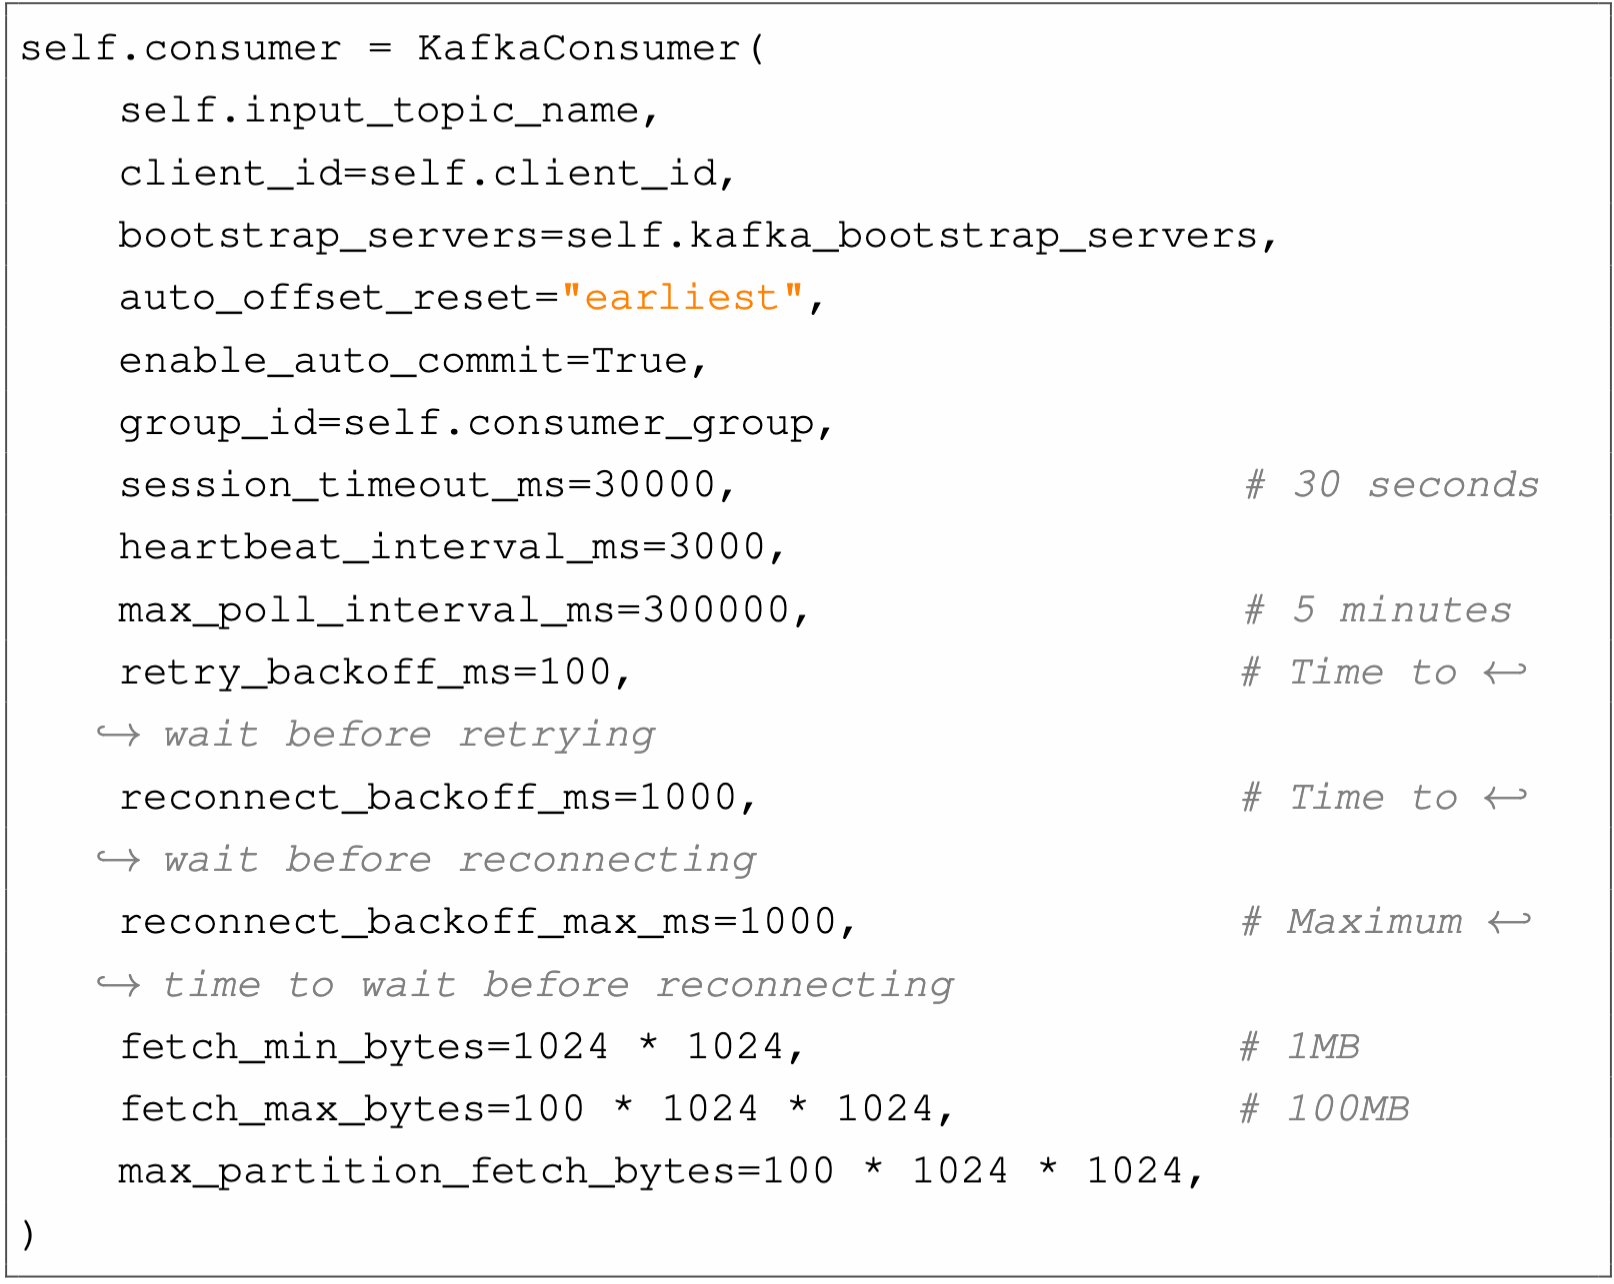
\includegraphics[width=1\textwidth]{Figure/consumer_conf.png}
    \caption{Kafka consumer configuration for centralized server.}
    \label{fig:consumer_config}
\end{figure}

The consumer configuration emphasizes parameters specific to server-side processing and high-volume data consumption:

\begin{itemize}
    \item \textbf{auto\_offset\_reset = ``earliest''}: Critical for Re-ID continuity—new consumer instances begin from the earliest available messages, ensuring no video frames are missed during consumer restarts or scaling operations.
    
    \item \textbf{enable\_auto\_commit = True}: Simplifies offset management for the idempotent Re-ID processing pipeline where occasional message reprocessing is acceptable compared to the complexity of manual offset management.
    
    \item \textbf{group\_id}: Enables horizontal scaling through consumer groups, allowing multiple server instances to process different partitions simultaneously while maintaining load balance across the Re-ID pipeline.
    
    \item \textbf{session\_timeout\_ms = 30000}: Extended 30-second timeout accommodates GPU-intensive operations (feature extraction, similarity searches) that may cause temporary processing delays, preventing unnecessary consumer group rebalancing.
    
    \item \textbf{heartbeat\_interval\_ms = 3000}: Maintains responsive group membership while staying well below the session timeout threshold, ensuring timely failure detection without overwhelming the cluster with heartbeat traffic.
    
    \item \textbf{max\_poll\_interval\_ms = 300000}: Allows 5-minute processing windows for complex Re-ID operations including vector database queries, similarity computations, and identity updates, preventing consumer eviction during intensive processing phases.
    
    \item \textbf{Fetch Configuration (fetch\_min\_bytes, fetch\_max\_bytes, max\_partition\_fetch\_bytes)}: Optimized for large video messages—minimum 1MB accumulation improves network efficiency while maximum 100MB limits prevent memory overflow. The increased partition fetch size (from default 1MB to 100MB) eliminates fetch size bottlenecks for HD video frames with detection metadata.
    
    \item \textbf{Reconnection Strategy (retry\_backoff\_ms, reconnect\_backoff\_*)}: Aggressive reconnection with minimal delays ensures rapid recovery for time-sensitive Re-ID processing where extended disconnections significantly impact tracking continuity.
\end{itemize}

This server-side configuration complements the edge device producer settings, creating an end-to-end optimized messaging pipeline that balances high-throughput video processing with the computational demands of real-time person re-identification.

\subsection{Configuration summary}

The following tables summarize the key configuration parameters for different components of the Kafka cluster deployment in the Re-ID system.

\subsubsection{Kafka Cluster and Topic Configuration}

\begin{table}[htbp]
\centering
\caption{Kafka Cluster and Topic Configuration}
\label{tab:kafka_cluster_config}
\begin{tabular}{|p{4cm}|p{8cm}|}
\hline
\textbf{Parameter} & \textbf{Value} \\
\hline
Topic Name & \texttt{reid\_input} \\
Number of Partitions & 6 \\
Replication Factor & 3 \\
Min In-Sync Replicas & 2 \\
Cleanup Policy & Delete \\
Retention Time & 1 day (86400000 ms) \\
Max Size on Disk & 20 GB \\
Maximum Message Size & 20 MB \\
\hline
Broker 1 & kafka1:29092 (Internal), :9092 (External) \\
Broker 2 & kafka2:29093 (Internal), :9093 (External) \\
Broker 3 & kafka3:29094 (Internal), :9094 (External) \\
Inter-Broker Protocol & PLAINTEXT \\
\hline
Zookeeper Connection & zookeeper:2181 \\
Zookeeper Configuration & Single node \\
\hline
\end{tabular}
\end{table}

\subsubsection{Producer Configuration (Edge Devices)}

\begin{table}[htbp]
\centering
\caption{Kafka Producer Configuration for Edge Devices}
\label{tab:producer_config}
\begin{tabular}{|p{4cm}|p{8cm}|}
\hline
\textbf{Parameter} & \textbf{Value} \\
\hline

Key Serializer & UTF-8 encoding for device identifiers \\
Value Serializer & Custom Avro-based serialization \\
Acknowledgment & \texttt{acks=1} (leader acknowledgment) \\
Batch Size & 16384 bytes (16 KB) \\
Linger Time & 10 ms (batch collection delay) \\
Max In-Flight Requests & 5 per connection \\
Partition Strategy & Round-robin distribution \\
\hline
\end{tabular}
\end{table}

\newpage

\subsubsection{Consumer Configuration (Central Server)}

\begin{table}[!htbp]
\centering
\caption{Kafka Consumer Configuration for Central Server}
\label{tab:consumer_config}
\begin{tabular}{|p{4cm}|p{8cm}|}
\hline
\textbf{Parameter} & \textbf{Value} \\
\hline
Auto Offset Reset & \texttt{earliest} (start from beginning) \\
Auto Commit & \texttt{True} (automatic offset management) \\
Group ID & Configurable consumer group identifier \\
Session Timeout & 30000 ms (30 seconds) \\
Heartbeat Interval & 3000 ms (3 seconds) \\
Max Poll Interval & 300000 ms (5 minutes) \\
Retry Backoff & 100 ms (minimal retry delay) \\
Reconnect Backoff & 1000 ms (1 second) \\
Fetch Min Bytes & 1024 KB (1 MB minimum fetch) \\
Fetch Max Bytes & 102400 KB (100 MB maximum fetch) \\
Max Partition Fetch & 102400 KB (100 MB per partition) \\
\hline
\end{tabular}
\end{table}